\documentclass[12pt,a4j]{jarticle}
\usepackage[dvipdfmx]{graphicx}
\begin{document}
\title{コンピュータリテラシレポート#13}
\author{1920031, 山川竜太郎}
\date{2019/07/19}
\maketitle


\section{課題の再掲}
( ここに課題の要約を記入 )

\section{レポートの本文}
( ここにレポートの本文を記入(適宜章立てを設定すると良い))

\begin{center}
  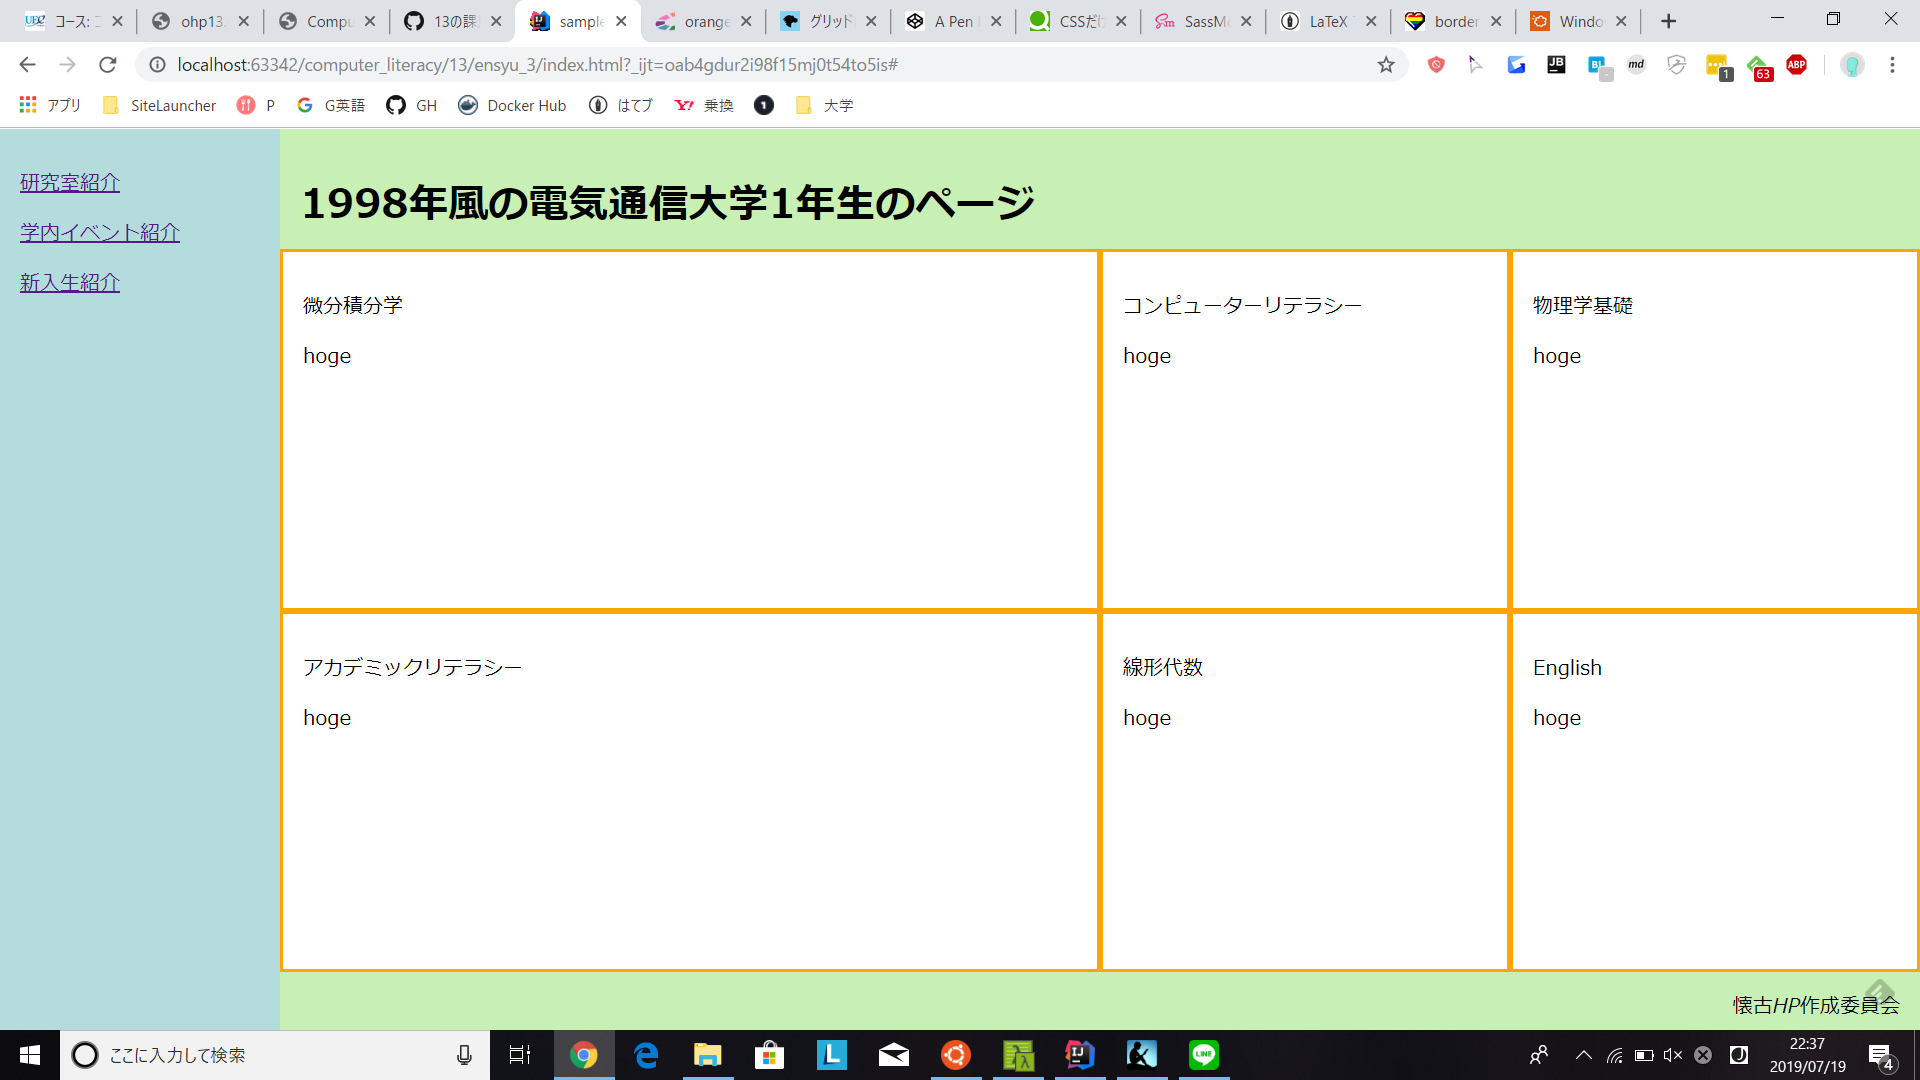
\includegraphics[width=10cm]{./ensyu_3/image.png}
\end{center}

\section{考察}
( ここに考察を記入 )

\section{アンケート}

\subsection{Q1:リンクや画像の使用についてどれくらい知っていましたか。}
( ここにQ1の回答を記入 )

\subsection{Q2:CSSによるブロックレイアウトについてはどうでしたか。どのようなページデザインがよいデザインだと思いますか。}
( ここにQ2の回答を記入 )

\subsection{Q3:リフレクション (今回の課題で分かったこと)・感想・要望をどうぞ。}
( ここにQ3の回答を記入 )

\end{document}
